

\tikzset{every picture/.style={line width=0.75pt}} %set default line width to 0.75pt        

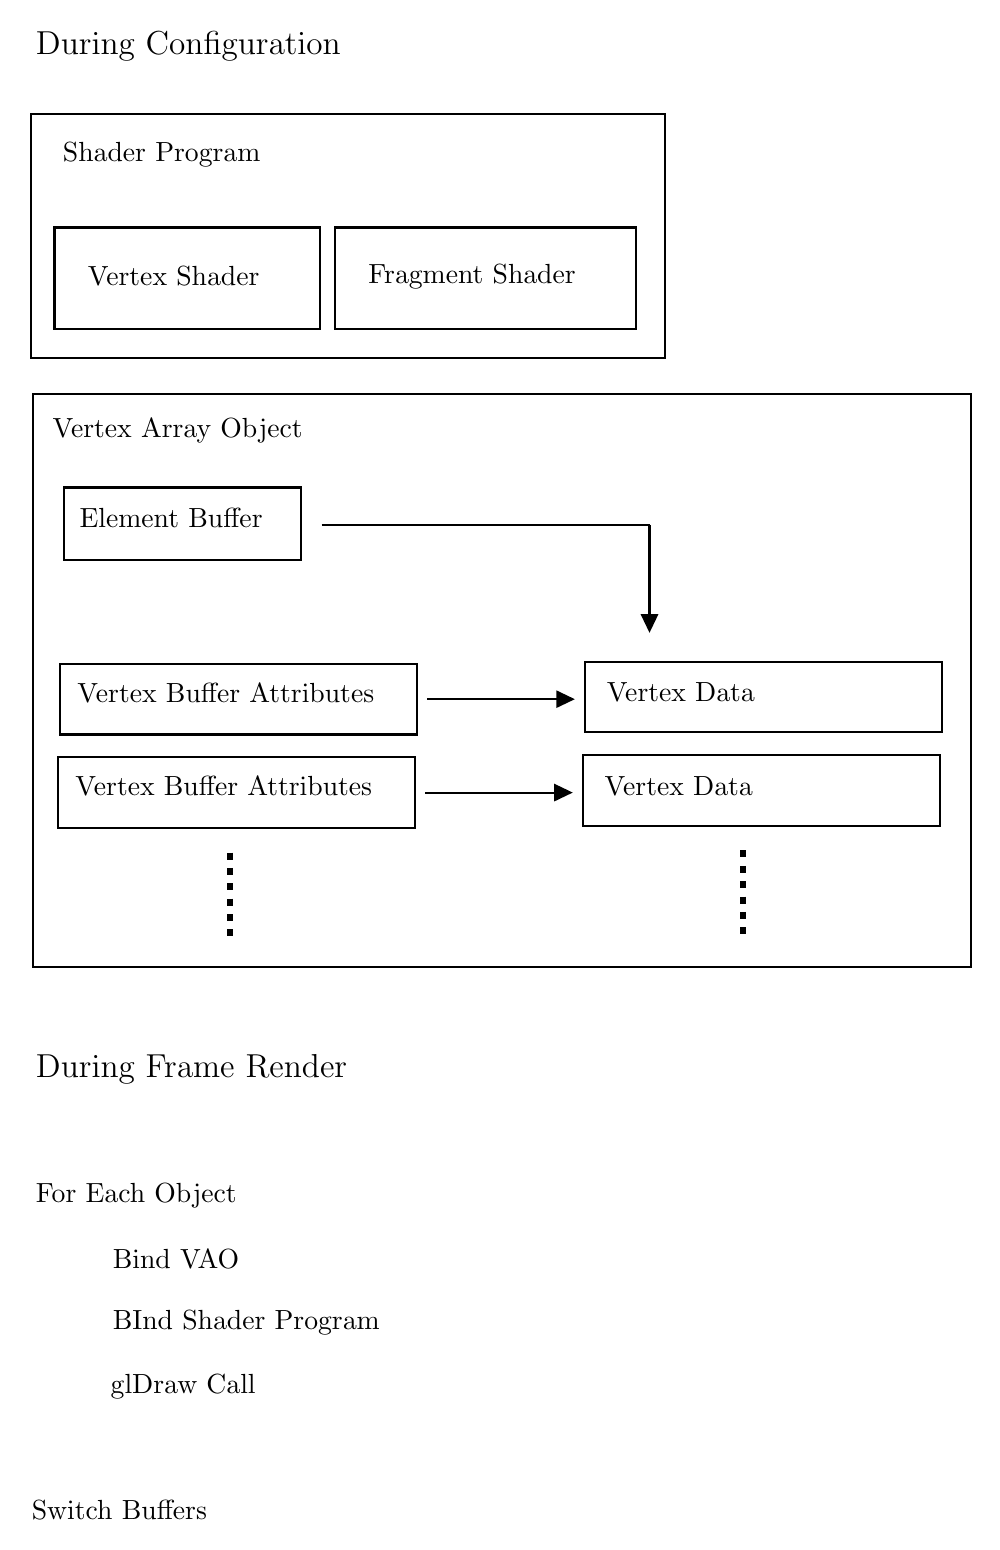
\begin{tikzpicture}[x=0.75pt,y=0.75pt,yscale=-1,xscale=1]
	%uncomment if require: \path (0,855); %set diagram left start at 0, and has height of 855
	
	%Shape: Rectangle [id:dp8822718697454482] 
	\draw   (94,64) -- (399.43,64) -- (399.43,181.77) -- (94,181.77) -- cycle ;
	%Shape: Rectangle [id:dp1908283304426488] 
	\draw   (105.43,118.77) -- (233.43,118.77) -- (233.43,167.77) -- (105.43,167.77) -- cycle ;
	
	%Shape: Rectangle [id:dp7244524197121301] 
	\draw   (240.43,118.77) -- (385.43,118.77) -- (385.43,167.77) -- (240.43,167.77) -- cycle ;
	
	%Shape: Rectangle [id:dp18755462550412272] 
	\draw   (95,199) -- (547.1,199) -- (547.1,475.03) -- (95,475.03) -- cycle ;
	%Shape: Rectangle [id:dp243965398016589] 
	\draw   (108,329) -- (280.1,329) -- (280.1,363.03) -- (108,363.03) -- cycle ;
	%Shape: Rectangle [id:dp6508857955705271] 
	\draw   (361,328) -- (533.1,328) -- (533.1,362.03) -- (361,362.03) -- cycle ;
	%Straight Lines [id:da5134438752708028] 
	\draw    (285.1,346.03) -- (353.1,346.03) ;
	\draw [shift={(356.1,346.03)}, rotate = 180] [fill={rgb, 255:red, 0; green, 0; blue, 0 }  ][line width=0.08]  [draw opacity=0] (8.93,-4.29) -- (0,0) -- (8.93,4.29) -- cycle    ;
	%Shape: Rectangle [id:dp19188267543228255] 
	\draw   (107,374) -- (279.1,374) -- (279.1,408.03) -- (107,408.03) -- cycle ;
	%Shape: Rectangle [id:dp3821137011287612] 
	\draw   (360,373) -- (532.1,373) -- (532.1,407.03) -- (360,407.03) -- cycle ;
	%Straight Lines [id:da7227305673378032] 
	\draw    (284.1,391.03) -- (352.1,391.03) ;
	\draw [shift={(355.1,391.03)}, rotate = 180] [fill={rgb, 255:red, 0; green, 0; blue, 0 }  ][line width=0.08]  [draw opacity=0] (8.93,-4.29) -- (0,0) -- (8.93,4.29) -- cycle    ;
	%Straight Lines [id:da408332221417708] 
	\draw [line width=2.25]  [dash pattern={on 2.53pt off 3.02pt}]  (190,419.93) -- (190,460.23) ;
	%Straight Lines [id:da06161874260645883] 
	\draw [line width=2.25]  [dash pattern={on 2.53pt off 3.02pt}]  (437,418.93) -- (437,459.23) ;
	%Shape: Rectangle [id:dp537977359727581] 
	\draw   (110.1,244.03) -- (224.1,244.03) -- (224.1,279.03) -- (110.1,279.03) -- cycle ;
	%Straight Lines [id:da7297870666377134] 
	\draw    (234.1,262.03) -- (392.1,262.03) ;
	%Straight Lines [id:da18316949817072714] 
	\draw    (392.1,262.03) -- (392.1,311.03) ;
	\draw [shift={(392.1,314.03)}, rotate = 270] [fill={rgb, 255:red, 0; green, 0; blue, 0 }  ][line width=0.08]  [draw opacity=0] (8.93,-4.29) -- (0,0) -- (8.93,4.29) -- cycle    ;
	
	% Text Node
	\draw (255.17,135) node [anchor=north west][inner sep=0.75pt]   [align=left] {Fragment Shader};
	% Text Node
	\draw (108,76) node [anchor=north west][inner sep=0.75pt]   [align=left] {Shader Program};
	% Text Node
	\draw (120,136) node [anchor=north west][inner sep=0.75pt]   [align=left] {Vertex Shader};
	% Text Node
	\draw (103,209) node [anchor=north west][inner sep=0.75pt]   [align=left] {Vertex Array Object};
	% Text Node
	\draw (115,336.73) node [anchor=north west][inner sep=0.75pt]   [align=left] {Vertex Buffer Attributes};
	% Text Node
	\draw (370,336.73) node [anchor=north west][inner sep=0.75pt]   [align=left] {Vertex Data};
	% Text Node
	\draw (114,381.73) node [anchor=north west][inner sep=0.75pt]   [align=left] {Vertex Buffer Attributes};
	% Text Node
	\draw (369,381.73) node [anchor=north west][inner sep=0.75pt]   [align=left] {Vertex Data};
	% Text Node
	\draw (116,252.73) node [anchor=north west][inner sep=0.75pt]   [align=left] {Element Buffer};
	% Text Node
	\draw (95,515.73) node [anchor=north west][inner sep=0.75pt]  [font=\large] [align=left] {During Frame Render};
	% Text Node
	\draw (95,23) node [anchor=north west][inner sep=0.75pt]  [font=\large] [align=left] {During Configuration};
	% Text Node
	\draw (132,609.73) node [anchor=north west][inner sep=0.75pt]   [align=left] {Bind VAO};
	% Text Node
	\draw (132,638.73) node [anchor=north west][inner sep=0.75pt]   [align=left] {BInd Shader Program};
	% Text Node
	\draw (95,577.73) node [anchor=north west][inner sep=0.75pt]   [align=left] {For Each Object};
	% Text Node
	\draw (131,669.73) node [anchor=north west][inner sep=0.75pt]   [align=left] {glDraw Call};
	% Text Node
	\draw (93,730.73) node [anchor=north west][inner sep=0.75pt]   [align=left] {Switch Buffers};
	
	
\end{tikzpicture}
